% Options for packages loaded elsewhere
\PassOptionsToPackage{unicode}{hyperref}
\PassOptionsToPackage{hyphens}{url}
%
\documentclass[
]{article}
\usepackage{amsmath,amssymb}
\usepackage{iftex}
\ifPDFTeX
  \usepackage[T1]{fontenc}
  \usepackage[utf8]{inputenc}
  \usepackage{textcomp} % provide euro and other symbols
\else % if luatex or xetex
  \usepackage{unicode-math} % this also loads fontspec
  \defaultfontfeatures{Scale=MatchLowercase}
  \defaultfontfeatures[\rmfamily]{Ligatures=TeX,Scale=1}
\fi
\usepackage{lmodern}
\ifPDFTeX\else
  % xetex/luatex font selection
\fi
% Use upquote if available, for straight quotes in verbatim environments
\IfFileExists{upquote.sty}{\usepackage{upquote}}{}
\IfFileExists{microtype.sty}{% use microtype if available
  \usepackage[]{microtype}
  \UseMicrotypeSet[protrusion]{basicmath} % disable protrusion for tt fonts
}{}
\makeatletter
\@ifundefined{KOMAClassName}{% if non-KOMA class
  \IfFileExists{parskip.sty}{%
    \usepackage{parskip}
  }{% else
    \setlength{\parindent}{0pt}
    \setlength{\parskip}{6pt plus 2pt minus 1pt}}
}{% if KOMA class
  \KOMAoptions{parskip=half}}
\makeatother
\usepackage{xcolor}
\usepackage[margin=1in]{geometry}
\usepackage{graphicx}
\makeatletter
\def\maxwidth{\ifdim\Gin@nat@width>\linewidth\linewidth\else\Gin@nat@width\fi}
\def\maxheight{\ifdim\Gin@nat@height>\textheight\textheight\else\Gin@nat@height\fi}
\makeatother
% Scale images if necessary, so that they will not overflow the page
% margins by default, and it is still possible to overwrite the defaults
% using explicit options in \includegraphics[width, height, ...]{}
\setkeys{Gin}{width=\maxwidth,height=\maxheight,keepaspectratio}
% Set default figure placement to htbp
\makeatletter
\def\fps@figure{htbp}
\makeatother
\setlength{\emergencystretch}{3em} % prevent overfull lines
\providecommand{\tightlist}{%
  \setlength{\itemsep}{0pt}\setlength{\parskip}{0pt}}
\setcounter{secnumdepth}{-\maxdimen} % remove section numbering
\usepackage{float}
\usepackage{sectsty}
\ifLuaTeX
  \usepackage{selnolig}  % disable illegal ligatures
\fi
\IfFileExists{bookmark.sty}{\usepackage{bookmark}}{\usepackage{hyperref}}
\IfFileExists{xurl.sty}{\usepackage{xurl}}{} % add URL line breaks if available
\urlstyle{same}
\hypersetup{
  hidelinks,
  pdfcreator={LaTeX via pandoc}}

\author{}
\date{\vspace{-2.5em}}

\begin{document}

\hypertarget{organism-physiology-in-response-to-multiple-drivers-of-environmental-change}{%
\section{Organism Physiology in Response to Multiple Drivers of
Environmental
Change}\label{organism-physiology-in-response-to-multiple-drivers-of-environmental-change}}

~~~~~ Organisms and environments are entwined, as the relationship
between organisms and the environments they are embedded within, is in
constant flux through inextricable links and flows of energy. The
relationship between organisms and environments varies through both
space and time and is influenced by a mosaic of dynamic biotic and
abiotic drivers \citep{connell1977mechanisms, menge1987community}.
Organisms are active participants in constructing their environment,
from altering seawater biogeochemistry through physiological processes
to organisms constructing biogenic structures; plenty of studies
demonstrate that the processes that organisms undergoe cascade to
influence the environment\citep{lewontin1983organism,estes1974sea}.
Organisms, throughout their development, must physiologically cope with
the conditions of the environment that they are situated within,
inlfuencing species beyond themselves and thus inevitably influencing
community structure and populations \citep{bozinovic2015physiological}.
Organisms and the ecosystems they construct, while playing an essential
role in structuring the physical and biological environment, are
simultaneously governed by the ability to perform and function under a
myriad of complex interactions, as each act to influence one another
non- contemporaneously and contemporaneously through direct and indirect
feedback loops \citep{levin1974disturbance,paine1980food}. Organisms are
simultaneously creators and products of the environment. In a geological
epoch of rapid ecological change, it is increasingly imperative to
understand the extent to which organisms can respond to environmental
variability across multiple drivers of change and how changing
organismal processes may scale up to influence other species.
Understanding physiological responses, interactions, and constraints of
marine organisms to anthropogenic climate change is perhaps the sine qua
non for understanding the changes between marine organisms and the
ecosystems they construct. This research intends to inform how the
changing oceanic environment may affect organismal physiology by teasing
apart the relationship between environmental drivers and physiological
performance to assess changes in energitic requirements. This research
also intends to elucidate how changes within physiological processes in
one organism may have indirect effects on other species. In this regard,
the fate of organisms is intertwined as the energetic requirements of
one species codetermines the other, illustrating that organisms are
directly or indirectly the subjects and objects of ecological change
\citep{lewontin1983organism}.

~~~~~ Environments undergo dynamic changes driven by natural
fluctuations in abiotic and biotic factors that, in turn, shape
community structure and processes, drive ecological shifts, and create
diverse mosaics of microhabitats
\citep{connell1961influence, stenseth2002ecological, kroeker2017embracing}.
Environmental drivers are an abiotic parameter that influences organisms
and environments across a spectrum ranging from enhancing, optimal, or
stressful conditions
\citep{cote2016interactions, boyd2012understanding}. For example, within
marine ecosystems, the combination of oceanographic processes and local
coastal geography may create an array of patterns and variability in
abiotic drivers such as temperature, flow, pH, dissolved oxygen, etc.,
that may impact the structure and processes of ecological communities on
distances ranging from microscale to macroscale
\citep{deser2010sea, hofmann2010living}. Such heterogeneous patterns are
naturally occurring and create complex gradients that shape ecological
communities and influence physiological processes within individual
organisms \citep{helmuth2006mosaic}.Many organisms have evolved to
withstand complex and variable environmental gradients, mediated through
physiological mechanisms such as phenotypic plasticity and
acclimatization \citep{hofmann2010living, tomanek2002heat}. According to
the metabolic theory of ecology, environmental gradients and changes in
abiotic factors may result in physiological trade-offs due to the
alterations within the energetic partitioning of an organism's
metabolism \citep{portner2008physiology, brown2004metabolic}.
Metabolism, comprises the total sum of biological and chemical processes
in converting energetic resources and materials into biomass and
activity \citep{brown2004metabolic}. Furthermore, organismal metabolic
rates are intrinsically linked to respiration rates, as cellular
respiration mediates the conversion of nutrients into energy in the form
of adenosine triphosphate (ATP) for cellular processes. By comparing the
respiration rates of organisms across gradients of environmental
drivers, we can effectively quantify and compare the metabolic
constraints and tolerance limits of organisms, thereby inferring changes
in energetic requirements as well as energetic transfer within
ecosystems \citep{somero2002thermal, silbiger2019comparative}. The
influence of multiple drivers of environmental change on metabolic
processes is of paramount interest in ecology, as alterations in
metabolism directly impact a species' survival, behavior, and energetic
requirements, consequently affecting fitness and ecosystem processes
\citep{carey2016sea}.

Cellular respiration involving the consumption of oxygen (O2) through a
process of organismal respiration to produce energy in the form of
adenosine triphosphate (ATP) \cite{babcock1992oxygen} according to the
equation:

\[
C_6H_{12}O_6 + 6O_2 \rightarrow 6CO_2 + 6H_2O + \text{energy (as ATP)}
\]

~~~~~ The physiological processes of marine organisms are directly
impacted by abiotic drivers such as temperature and pH, which play
pivotal roles in shaping the functioning and structure of marine
ecosystems. \citep{woodwell1970effects}. Temperature, in particular, is
the fundamental driver in determining physiological rates of organisms
as the kinetic energy of biochemical reactions is temperature dependent
\citep{levins1968evolution, somero2002thermal, portner2012integrating}.
Biological processes such as organismal and ecological interactions are
also strongly influenced by temperature
\citep{hochachka2002biochemical}. This is exemplified by the
relationship between temperature and body size, where organisms develop
faster yet decrease in size under elevated temperatures
\citep{elahi2020historical}. Metabolic rates are strongly influenced by
an organism's body size and temperature and are subject to change due to
changes in abiotic drivers and the natural variability of drivers
\citep{brown2004metabolic, oconnor2007temperature}. Further, organisms
adapt to local temperatures to match optimal conditions for
physiological processes and acclimatize to a range around these values
\citep{sinclair2016can}. Any range too far beyond the ability of an
organism to acclimatize influences survival, fitness, and population
densities \citep{hochachka2002biochemical}. Studies have shown the
influence of sea surface temperature on metabolic processes such as
growth, feeding, reproduction, and influencing the range of species
distributions
\citep{kordas2011community, sanford2002feeding, pinsky2013marine}.
However, it is essential to note that temperature is not the only driver
of biological processes and temperature has interactive effects with
other abiotic drivers \citep{darling2008quantifying}. pH is also an
important abiotic driver that impacts the physiological performance of
marine organisms and influences the biogenic structures that organisms
create \citep{hofmann2010living}. pH plays a vital role in metabolic
processes due to its effect on biochemical pathways and internal
acid-base balance \citep{gaylord2015ocean}. For example, low pH is often
associated with elevated metabolic rates due to the increase in
energetic costs in creating calcified structures such as the formation
of shells in mollusks or the skeletons of corals and echinoderms
\citep{doney2009ocean, spalding2017energetic}. Due to differences in the
energetic costs associated with calcification, there are significant
differences in the ability to control acid-base regulation between
species \citep{doney2009ocean}. Consequently, changes in physicochemical
parameters of the environment affect species differently, impact the
interaction between species and, in turn, affect the structures of
ecological communities; therefore, studying how differences between
abiotic drivers affect organismal physiology will have ecosystem-level
implications \citep{tomanek2002physiological, barclay2019variation}.

~~~~~ Organisms are adapted to cope with a natural range of abiotic
conditions, yet anthropogenic climate change may outpace organismal
physiological capacities and may also act interactively to result in
``ecological surprises'\,' (sense, Paine et al., 1969). For example, the
cumulative impact of two drivers acting together may interact to be
equivalent to their sum, known as an additive effect, less than their
additive effect, which is known as an antagonistic interaction, or
greater than their additive effect, known as a synergistic interaction
(Côté et al., 2016). For decades anti-racist and feminist scholars have
provided critical insight into the ways in we must think about isolated
phenomena as intersectional due to their complex interactions (Davis,
1983; Crenshaw, 1989). The field of marine biology requires this
paradigm shift that embraces the interactions between stressors to grasp
the complexity of the future. Combined, these drastic changes in abiotic
drivers will continue to act in conjecture with one another and could
potentially ameliorate or exacerbate impacts on organismal physiological
processes and reverberate the effects of ecological change through
ecosystems (Kroeker, Kordas, \& Harley, 2017).

\newpage

~~~~~ As the atmospheric carbon dioxide (CO2) concentration continues to
surpass the limits of the earth system, marine organisms will be forced
to endure profound transformations of the environment, from shifts in
temperature to altered geochemistry (richardson2023earth,
portner2008physiology\}. Ocean warming (OW) and ocean acidification (OA)
represent two of the most significant changes occurring in marine
ecosystems across the globe, both driven by the unremitted rise of
anthropogenic-induced carbon dioxide emissions. OW and OA are not
isolated phenomena; they share a common origin, and in a rapidly
changing world, their combined impacts on organismal physiology
necessitate special attention as multiple drivers of change may act
interactively \citep{cote2016interactions}. Since the beginning of the
20th century, the global mean sea surface temperature (SST) has
increased by 0.88 {[}0.68--1.01{]}\(^\circ\)C, and is further projected
to warm by 2.89\(^\circ\)C {[}2.01--4.07\(^\circ\)C{]} at the end of the
century, which surpasses the thermal tolerance limits of many marine
species (following the representative concentration pathway 8.5 emission
scenario)
\citep{kikstra2022ipcc, fox2021ocean, bay2017genomic, somero2010physiology}.
Concurrently, the ocean has absorbed \textasciitilde30\% of
anthropogenic CO2 \citep{feely2004impact}, altering the carbonate
chemistry of seawater through a decrease in the concentration of
carbonate ions \(\mathrm{CO_3^{2-}}\) and a decline in seawater pH
\citep{feely2004impact}. Mean surface ocean pH values have declined by
0.1 units since the pre-industrial era, with a further projected
diminution of 0.1 - 0.4 units by the end of the century
\citep{change2014impacts, orr2005anthropogenic}, posing a unique threat
to calcifying marine organisms. Consequently, the impacts of OW and OA
will not be consistent across geographic regions, leading to
differential effects that will modify already variable spatial and
temporal environments. Building a mechanistic understanding of how the
combined impacts of ocean warming and acidification affect marine
organisms is integral for reliable projections of how climate change may
continue to affect marine organisms.

~~~~~ Coastal marine organisms frequently encounter a wide range of
temperatures and experience fluctuations in biogeochemistry, resulting
from temporal variations, such as tidal and seasonal cycles. The rocky
intertidal system is one such system that is known for its variable
conditions on both temporal and spatial scales, making them a model
ecosystem for understanding how organisms interact and respond to change
\citep{connell1961influence, paine1969pisaster, kwiatkowski2016nighttime, jellison2022low}.
Organisms within the rocky intertidal zone must contend with alternating
periods of immersion and emersion of tidal fluctuations, which commonly
lead to large variations in temperature, oxygen availability, and pH,
\citep{denny2001physical, helmuth2002climate}. Of these naturally
occurring changes, thermal variability within the intertidal zone is
believed to be a dominant driver in structuring the vertical and
latitudinal distribution patterns by limiting upper zonation through
abiotic stress and lower zonation through biotic influence
\citep{helmuth2006mosaic, somero2002thermal, somero2010physiology, connell1961influence}.
Daily temperature fluctuations are drastic enough to elevate the body
temperatures of marine organisms by more than 20\(^\circ\)C during a
tidal emersion event \citep{Helmuth1999thermal}. Furthermore, changes in
pH within tidepools may exceed 1 unit when nighttime respiration rates
exceed photosynthetic rates
\citep{jellison2016ocean, kwiatkowski2016nighttime}. Such highly
variable abiotic changes are naturally occurring and create complex
gradients that shape ecological communities and influence physiological
processes within individual organisms \citep{helmuth2006mosaic}. Given
that organisms within the intertidal zone simultaneously face drastic
fluctuations from abiotic drivers, and experience conditions far beyond
what is expected in the future, understanding organismal performance in
these ecosystems may provide a window for looking toward the future.
Intertidal organisms are well known for the ability to utilize anaerobic
metabolic responses (e.g., metabolic depression) to minimize metabolic
costs of dealing with thermal stress, making them an ideal model system
to understand the impacts of thermal stress on physiology (Pörtner et
al., 2017).

~~~~~ The role of biotic and abiotic drivers in influencing metabolic
processes has been of primary interest to the field of ecology as
changes in metabolism directly affect the survival, behavior, and energy
requirements of organisms, thereby impacting organism and ecosystem
function \citep{carey2016sea}. Physiological processes are heavily
influenced by environmental factors, and many marine organisms undergo
biological responses to natural diel variability present within
environments \citep{hofmann2010living}. Temperature is the primary
environmental driver regulating physiological rates of ectothermic
organisms, as kinetic energy of biochemical reactions are temperature
dependent
\citep{levins1968evolution, huey1979integrating, hochachka2002biochemical}.
Further, temperature is the key determinant in the regulating rates of
biological processes, ranging from metabolic rates
\citep{gillooly2001effects} to species interactions
\citep{sanford1999regulation}, such as growth, feeding, reproduction,
and determining the range of species distributions
\citep{kordas2011community, sanford2002feeding, pinsky2013marine}. The
physiological processes of metabolism are the total sum of biological
and chemical processes in converting energetic resources and materials
into biomass and activity \citep{brown2004metabolic}. Changes in pH also
play a vital role in metabolic processes due to its effect on
biochemical pathways and internal acid-base balance
\citep{gaylord2015ocean}. Specifically, declines in seawater carbonate
ions and pH attributed to OA are strongly correlated to decreases in
calcification and growth rates of many marine organisms
\citep{kroeker2013impacts}. Due to species-specific differences in the
energetic costs associated with calcification, there are significant
differences in the ability to control internal acid-base regulation
between species \citep{doney2009ocean}. Ultimately, changes in the
environment that lead to alterations in organismal energetic
requirements will scale up to affect the processes of ecological
communities; therefore, studying how multiple abiotic factors affect
organismal physiology has ecosystem-level implications
\citep{tomanek2002heat, barclay2019variation, kroeker2022ecological}.

\newpage

\hypertarget{thermal-performance-curves-as-a-tool-to-understand-multiple-drivers-of-change-on-organismal-physiology}{%
\subsection{Thermal Performance Curves as a Tool to Understand Multiple
Drivers of Change on Organismal
Physiology}\label{thermal-performance-curves-as-a-tool-to-understand-multiple-drivers-of-change-on-organismal-physiology}}

\begin{figure}[htbp]
    \centering
    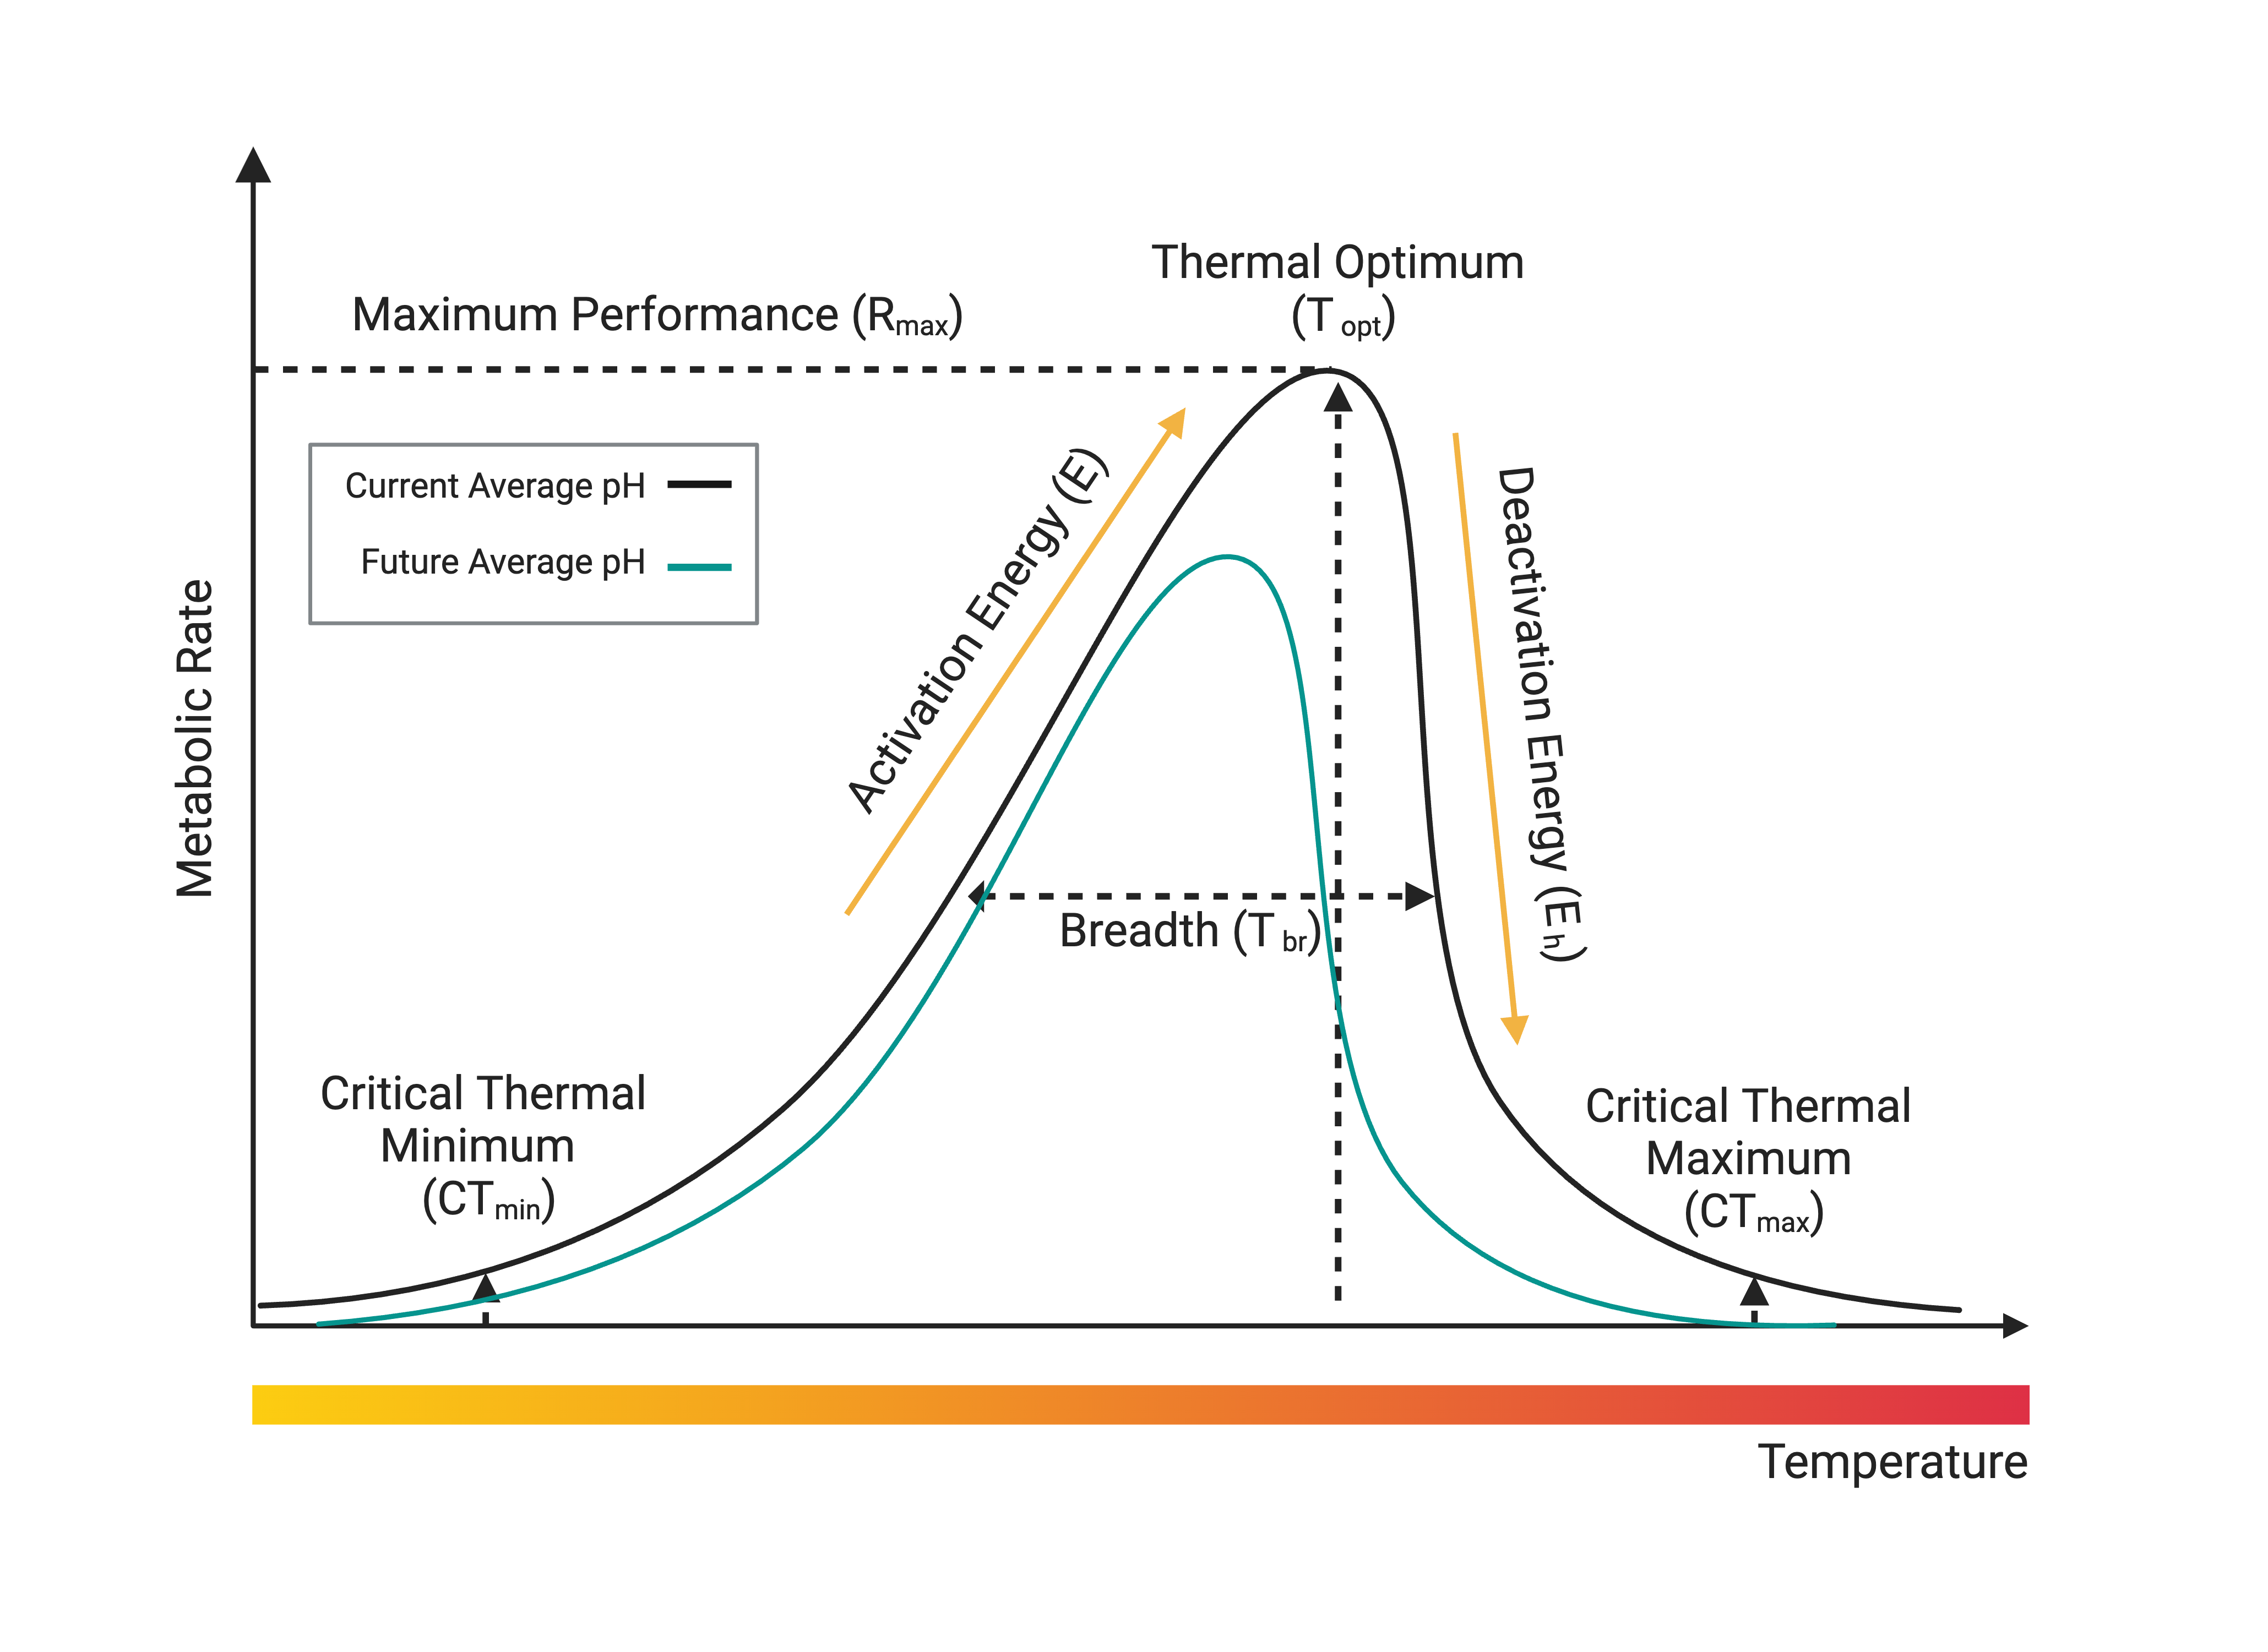
\includegraphics[width=1\textwidth]{Images/thermal_performance_curve_schematic.png}
    \caption{Figure 1. Thermal performance curve schematic illustrating the relationship between biological rates and temperature, including critical thermal maximum (CTMax), critical thermal minimum (CTMin), thermal optimum (Topt), activation energy (E), deactivation energy (Eh), and the thermal breadth of the curve (TBr). Hypothesized characteristics of a thermal performance curve exposed to ocean acidification, including reduced thermal optimum, reduced performance of maximum physiological rate, and reduced breathe of the curve.}
    \label{fig:thermal-performance-curve-schematic}
\end{figure}

~~~~~ The use of performance curves can help to quantify the
relationship between abiotic drivers and physiological rates to forecast
future effects \cite{kroeker2017embracing} and can allow for comparative
assessments across different biological rates and environmental
conditions (Figure 1.)
\cite{schulte2011thermal, silbiger2019comparative, silva2021local, padfield2021rtpc, becker2020nutrient}.
Further, thermal performance curves have been suggested to fill in the
gap of uncertainty between multiple stressors as they empirically
characterize the relationship between biological performance rates
across a wide range of temperatures
\cite{padfield2021rtpc, schulte2011thermal, silbiger2019comparative}.
Thermal performance curves are a univariate function that describes how
some measure of performance (e.g., metabolic rate) varies with
temperature. As temperature increases so do the biochemical and
physiological rates until they reach a species-specific optimal
temperature. Beyond the optimum rate, further increases in temperature
denature proteins, stunt growth, and cause reductions in performance and
survival \cite{somero2002thermal, portner2002climate}. Thermal
performance curves are typically left-skewed and hump-shaped and include
several metrics, including but not limited to a thermal optimum
(TOpt)---the temperature at the highest rate of performance---and a
critical thermal minimum (CTMin) and a thermal maximum (CTMax)--- the
upper and lower thermal limit that an organism can tolerate
\cite{schulte2011thermal, huey1979integrating, huey1989evolution}. These
tolerance thresholds and the range they encompass are governed by an
organism's ability to respond to sub-lethal and lethal conditions
through an organismal-level response and molecular-level responses such
as anaerobic metabolism and heat shock response
\cite{portner2017oxygen, somero2002thermal}. Further, exposure to
concurrent drivers of ecological change, like OA, are expected to
constrict an organism's performance curve and thermal limits, such as
decreasing the breadth of thermal performance
\cite{portner2008physiology, portner2010oxygen}. Comparing physiological
responses to gradients of abiotic drivers may allow us to quantify and
compare the tolerance limits of organisms
\cite{silbiger2019comparative}.

~~~~~ Despite the increasing emphasis on multi-driver and multi-species
studies, a mechanistic understanding of the nonlinear responses of
multiple confounding stressors of future scenarios remains a knowledge
gap. (Kroeker, Kordas, \& Harley, 2017). The elevated sense of urgency
involved with these global threats contributes to the need for a more
nuanced understanding of the impact of multiple stressor interactions on
organismal and ecosystem processes (Côté et al., 2016). The response of
organisms to climate change, survival, and fitness depends on
physiological trade-offs, which are essentially changed within the
allocation of an organism's energy for different biological functions
and demands for resources. Considering that metabolic processes respond
differently to multiple environmental drivers and that physiological
systems within and between organisms differ, it is imperative to tease
apart the metabolic rates. Organisms may respond to changing abiotic
drivers by altering their energetic allocation or energetic intake, such
as altering consumption rates or growth (O'Connor 2009). For example,
the metabolic theory of ecology predicts an increase in consumption
rates with increasing temperature (O'Connor 2009). These alterations
within an individual species' physiological performance are significant
because they can scale up to affect ecosystem function (Post et al.,
1999). Building a mechanistic understanding regarding how the combined
impacts of ocean warming and acidification affect marine organisms is
integral for reliable projections of how climate change may continue to
affect marine organisms.

~~~~~ Specifically, we ask the question: how does exposure to decreased
pH influence thermal performance curves of respiration of an intertidal
gastropod, Tegula funebralis? We anticipate that the thermal optimum
(TOpt) for respiration rates will shift towards lower temperatures,
indicating a reduced ability to sustain optimal metabolic activity in
the face of ocean acidification. Additionally, we expect a decrease in
the thermal breadth of the curve (TBr), indicating a narrower range of
temperatures at which the gastropod can effectively maintain its
respiratory rates.

\end{document}
